\chapter{DNA: एक सार्वत्रिक आनुवंशिक अणु}\label{ch:g10:universal-dna}

अँधेरी प्रयोगशाला में, नीले लैंप के नीचे, दो सफ़ेद चूहों में से एक नाक
से पूँछ तक हरा चमक रहा है। वह अपनी हर \omterm{def:g10:cells-common-unit:cell}{कोशिका} में प्रशांत महासागर में
चमकने वाली एक जेलीफ़िश से लिया गया अकेला एक \omterm{def:g10:universal-dna:gene}{जीन} ढोता है --- और चूहे की
\omterm{def:g10:cells-common-unit:cell}{कोशिकाएँ} जेलीफ़िश के उस \omterm{def:g10:universal-dna:gene}{जीन} को ठीक वैसे ही पढ़ती हैं जैसे ख़ुद
जेलीफ़िश की \omterm{def:g10:cells-common-unit:cell}{कोशिकाएँ}। यह प्रयोग इसलिए चलता है कि हर सजीव अपने \omterm{def:g10:universal-dna:gene}{जीन} उसी एक
अणु में, उन्हीं चार अक्षरों से लिखता है और उन्हें उन्हीं नियमों से पढ़ता
है। यह अध्याय उसी अणु, यानी \omterm{def:g10:universal-dna:information}{DNA}, के बारे में है: वह बना कैसे है, उसकी
बनावट क्या-क्या समझाती है, और वह चमकता चूहा क्या सिद्ध करता है।

\section{आनुवंशिक पदार्थ}

\begin{definition}[आनुवंशिक जानकारी]\label{def:g10:universal-dna:information}
किसी \omterm{def:g10:cells-common-unit:cell}{कोशिका} की \emph{आनुवंशिक जानकारी}\index{आनुवंशिक जानकारी} निर्देशों
का वह समुच्चय है जो \omterm{def:g10:cells-common-unit:cell}{कोशिका} से उसकी पुत्री \omterm{def:g10:cells-common-unit:cell}{कोशिकाओं} तक और जनकों से संतान
तक पहुँचता है और जो जीव के लक्षण तथा उसकी \omterm{def:g10:cells-common-unit:cell}{कोशिकाओं} के बना सकने वाले
\omterm{def:g10:chemistry-of-life:families}{प्रोटीन} तय करता है। हर सजीव में उसे \emph{DNA}\index{DNA}
(डिऑक्सीराइबोन्यूक्लिक अम्ल) के अणु ढोते हैं, जो प्रोटीनों के साथ कसकर
\emph{गुणसूत्रों}\index{गुणसूत्र} में बँधे रहते हैं --- \omterm{def:g10:cells-common-unit:prokaryote}{सुकेंद्रकी
कोशिका} में \omterm{def:g10:cells-common-unit:organelle}{केंद्रक} के भीतर, और जीवाणु में \omterm{def:g10:cells-common-unit:cell}{कोशिकाद्रव्य} में खुले।
\end{definition}

\begin{proposition}[DNA ही आनुवंशिकता का अणु है]\label{prop:g10:universal-dna:material}
किसी \omterm{def:g10:cells-common-unit:cell}{कोशिका} का वंशागत पदार्थ उसका \omterm{def:g10:universal-dna:information}{DNA} है, न कि उसके \omterm{def:g10:chemistry-of-life:families}{प्रोटीन} या कोई और
घटक: शुद्ध किया गया \omterm{def:g10:universal-dna:information}{DNA} जीवाणुओं के एक प्रभेद से दूसरे में पहुँचाने पर
पहले प्रभेद के लक्षण भी साथ पहुँच जाते हैं।
\end{proposition}
\begin{proof}[साक्ष्य]
ग्रिफ़िथ (1928) ने पाया कि निमोनिया के हानिरहित जीवाणु किसी घातक प्रभेद
की मारी हुई \omterm{def:g10:cells-common-unit:cell}{कोशिकाओं} के साथ मिलाने पर ख़ुद घातक हो गए और पीढ़ियों तक
वैसे ही बने रहे: मरी हुई \omterm{def:g10:cells-common-unit:cell}{कोशिकाओं} की किसी चीज़ ने उन्हें
``रूपांतरित'' कर दिया था। एवरी, मैक्लॉड और मैक्कार्टी (1944) ने मरी हुई
\omterm{def:g10:cells-common-unit:cell}{कोशिकाओं} के सत्त को उसके अणु-कुलों में अलग किया और हर एक को परखा: केवल
\omterm{def:g10:universal-dna:information}{DNA} वाला अंश रूपांतरित करता था; \omterm{def:g10:universal-dna:information}{DNA} को नष्ट करने वाले एंजाइम से सत्त का
उपचार करने पर असर ख़त्म हो गया, जबकि \omterm{def:g10:chemistry-of-life:families}{प्रोटीन} या RNA नष्ट करने वाले
एंजाइमों से नहीं। तो रूपांतरित करने वाला पदार्थ, और इसलिए वंशागत लक्षण का
वाहक, \omterm{def:g10:universal-dna:information}{DNA} था।
\end{proof}

\begin{example}[DNA है कहाँ]\label{ex:g10:universal-dna:where}
\omterm{def:g10:universal-dna:information}{DNA} के लिए विशिष्ट कोई रंजक गाल की \omterm{def:g10:cells-common-unit:cell}{कोशिका} के \omterm{def:g10:cells-common-unit:organelle}{केंद्रक} को रँगता है और
\omterm{def:g10:cells-common-unit:cell}{कोशिकाद्रव्य} में और कुछ नहीं; विभाजित होती \omterm{def:g10:cells-common-unit:cell}{कोशिका} में वह सघन \omterm{def:g10:universal-dna:information}{गुणसूत्रों}
को रँगता है। जीवाणु उस रंजक को बिना किसी लिफ़ाफ़े वाले एक केंद्रीय
क्षेत्र में ग्रहण करता है। दोनों में \omterm{def:g10:universal-dna:information}{DNA} की मात्रा हर विभाजन से पहले
दोगुनी होती है और दोनों पुत्री \omterm{def:g10:cells-common-unit:cell}{कोशिकाओं} के बीच आधी-आधी बँट जाती है ---
यानी ठीक वह व्यवहार जिसकी उम्मीद उस जानकारी से की जाती है जिसकी नक़ल
बनाकर उसे बाँटना है।
\end{example}

\section{DNA की बनावट}

\begin{definition}[न्यूक्लियोटाइड]\label{def:g10:universal-dna:nucleotide}
\omterm{def:g10:universal-dna:information}{DNA} \emph{न्यूक्लियोटाइडों}\index{न्यूक्लियोटाइड} की एक शृंखला है। हर
न्यूक्लियोटाइड तीन हिस्सों से बना है: एक फ़ॉस्फ़ेट समूह, एक शर्करा
(डिऑक्सीराइबोस) और नाइट्रोजनयुक्त चार में से एक
\emph{क्षारक}\index{क्षारक (DNA)}: एडेनीन (A), थाइमीन (T), ग्वानीन (G)
और साइटोसीन (C)। शर्कराएँ और फ़ॉस्फ़ेट बारी-बारी से आकर शृंखला की रीढ़
बनाते हैं; क्षारक उससे बाहर निकले रहते हैं, हर न्यूक्लियोटाइड पर एक।
चारों न्यूक्लियोटाइड केवल अपने क्षारक से अलग हैं, इसलिए \omterm{def:g10:universal-dna:information}{DNA} की किसी लड़ी
का वर्णन उसके क्षारकों के अनुक्रम से किया जाता है, जिसे अक्षरों की एक
माला की तरह लिखा जाता है: \texttt{ATGGCTTAC\dots}
\end{definition}

\begin{omfigure}
\begin{tikzpicture}[>=Stealth, font=\small]
  % left strand backbone
  \foreach \i in {0,...,5} {
    \draw[fill=gray!30] (0,{1.1*\i}) circle (0.22);           % phosphate
    \draw[fill=omDef!25] (0.9,{1.1*\i+0.15}) -- (1.35,{1.1*\i+0.45}) -- (1.35,{1.1*\i-0.15}) -- (0.9,{1.1*\i-0.45}) -- (0.55,{1.1*\i}) -- cycle; % sugar (pentagon)
    \draw (0.22,{1.1*\i}) -- (0.55,{1.1*\i});
    \draw (1.35,{1.1*\i+0.45}) -- (0,{1.1*\i+1.1-0.22});
  }
  \foreach \i in {0,...,5} {
    \draw[fill=gray!30] (7.6,{1.1*\i+0.55}) circle (0.22);
    \draw[fill=omDef!25] (6.7,{1.1*\i+0.55+0.15}) -- (6.25,{1.1*\i+0.55+0.45}) -- (6.25,{1.1*\i+0.55-0.15}) -- (6.7,{1.1*\i+0.55-0.45}) -- (7.05,{1.1*\i+0.55}) -- cycle;
    \draw (7.38,{1.1*\i+0.55}) -- (7.05,{1.1*\i+0.55});
  }
  \foreach \i in {0,...,4}
    \draw (6.25,{1.1*\i+0.55+0.45}) -- (7.6,{1.1*\i+0.55+1.1-0.22});
  % base pairs
  \foreach \i/\l/\r/\cl/\cr in {0/A/T/omThm/omMeth, 1/G/C/omProp/omDef,
      2/C/G/omDef/omProp, 3/T/A/omMeth/omThm, 4/A/T/omThm/omMeth, 5/G/C/omProp/omDef} {
    \draw[fill=\cl!40] (1.35,{1.1*\i+0.15-0.25}) rectangle (3.7,{1.1*\i+0.15+0.25});
    \node at (2.5,{1.1*\i+0.15}) {\l};
    \draw[fill=\cr!40] (3.9,{1.1*\i+0.15-0.25}) rectangle (6.25,{1.1*\i+0.15+0.25});
    \node at (5.1,{1.1*\i+0.15}) {\r};
    \draw[densely dotted, thick] (3.7,{1.1*\i+0.15}) -- (3.9,{1.1*\i+0.15});
  }
  \node[anchor=east, align=right] at (-0.4,2.9) {फ़ॉस्फ़ेट और\\ शर्करा की\\ रीढ़};
  \node[anchor=west, align=left] at (8.0,3.45) {दूसरी\\ लड़ी};
  \node[anchor=south] at (2.5,6.5) {क्षारक, जोड़ों में};
  \draw[->] (0,-0.5) -- (0,-1.0) node[below] {लड़ी 1 की दिशा};
  \draw[->] (7.6,0.05) -- (7.6,-1.0) node[below] {लड़ी 2, उल्टी दिशा};
  \draw[<->, thick] (8.9,0.15) -- (8.9,1.25) node[midway, right] {\qty{0.34}{nm}};
\end{tikzpicture}

{\small \omterm{def:g10:universal-dna:information}{DNA} की दोनों लड़ियाँ, चपटी खींची हुई। हर लड़ी \omterm{def:g10:universal-dna:nucleotide}{न्यूक्लियोटाइडों}
(फ़ॉस्फ़ेट, शर्करा, \omterm{def:g10:universal-dna:nucleotide}{क्षारक}) की एक शृंखला है। दोनों लड़ियाँ उल्टी दिशाओं
में चलती हैं और क्षारक-जोड़ों से आपस में बँधी रहती हैं: A हमेशा T के
सामने, G हमेशा C के सामने। हर \qty{0.34}{nm} पर अगला क्षारक-जोड़ा आता है।}
\end{omfigure}

\begin{proposition}[द्विकुंडली]\label{prop:g10:universal-dna:helix}
\omterm{def:g10:universal-dna:information}{DNA} का अणु दो लड़ियों से बना है जो एक-दूसरे के चारों ओर लगभग \qty{2}{nm}
चौड़ी दक्षिणावर्त \emph{द्विकुंडली}\index{द्विकुंडली} में लिपटी रहती
हैं, और हर दस क्षारक-जोड़ों (\qty{3.4}{nm}) पर एक चक्कर पूरा होता है।
दोनों लड़ियाँ उल्टी दिशाओं में चलती हैं और अपने \omterm{def:g10:universal-dna:nucleotide}{क्षारकों} से एक-दूसरे के
सामने रहती हैं, जो \emph{पूरकता}\index{पूरकता} के एक कड़े नियम से जोड़े
बनाते हैं: A केवल T के साथ, G केवल C के साथ। इसलिए एक लड़ी का अनुक्रम
दूसरी का अनुक्रम तय कर देता है।
\end{proposition}
\begin{proof}[साक्ष्य]
शारगाफ़ (1950) ने बहुत-सी जातियों के \omterm{def:g10:universal-dna:information}{DNA} का क्षारक-संघटन मापा और हर एक
में A जितना T और G जितना C पाया, जबकि A+T और G+C का अनुपात जाति-दर-जाति
बदलता था --- यानी यह कोई रासायनिक संयोग नहीं, एक जोड़ी बनाने का नियम था।
फ़्रैंकलिन के \omterm{def:g10:universal-dna:information}{DNA} तंतुओं के एक्स-किरण चित्रों (1952) ने \qty{2}{nm} व्यास
और \qty{3.4}{nm} चक्कर वाली कुंडली के लक्षण दिखाए। वाटसन और क्रिक (1953)
ने वही अकेला मॉडल बनाया जो दोनों पर खरा उतरता है: दो रीढ़ें बाहर, जुड़े
हुए \omterm{def:g10:universal-dna:nucleotide}{क्षारक} भीतर, और A--T तथा G--C जोड़े एक ही चौड़ाई के, ताकि कुंडली
नियमित रहे।
\end{proof}

\begin{example}[अंकों में शारगाफ़ का नियम]\label{ex:g10:universal-dna:chargaff}
मानव \omterm{def:g10:universal-dna:information}{DNA}: A 30.9\%, T 29.4\%, G 19.9\%, C 19.8\% --- यानी माप की
यथार्थता के भीतर A$\,\approx\,$T और G$\,\approx\,$C, और
A+T $= 60\%$। \emph{E.~coli}: A 24.7\%, T 23.6\%, G 26.0\%, C 25.7\%,
A+T $= 48\%$। खमीर: A+T $= 64\%$। यदि किसी \omterm{def:g10:universal-dna:information}{DNA} नमूने में 32\% A हो, तो
\omterm{prop:g10:universal-dna:helix}{पूरकता} से 32\% T और G तथा C में से हर एक का $(100 - 64)/2 = 18\%$
निकलता है।
\end{example}

\begin{omfigure}
\begin{tikzpicture}
\begin{axis}[
  ybar, bar width=7pt,
  width=0.86\linewidth, height=5.4cm,
  axis x line=bottom, axis y line=left,
  ymin=0, ymax=40, ylabel={क्षारकों का \%}, ylabel style={font=\small},
  symbolic x coords={मनुष्य, खमीर, E. coli, गेहूँ},
  xtick=data, tick label style={font=\small},
  enlarge x limits=0.18,
  legend style={at={(0.5,-0.2)}, anchor=north, legend columns=4,
                font=\small, draw=none},
]
\addplot[fill=omThm!50, draw=omThm] coordinates {(मनुष्य,30.9) (खमीर,31.3) (E. coli,24.7) (गेहूँ,27.3)};
\addplot[fill=omMeth!60, draw=omMeth] coordinates {(मनुष्य,29.4) (खमीर,32.9) (E. coli,23.6) (गेहूँ,27.1)};
\addplot[fill=omProp!50, draw=omProp] coordinates {(मनुष्य,19.9) (खमीर,18.7) (E. coli,26.0) (गेहूँ,22.7)};
\addplot[fill=omDef!50, draw=omDef] coordinates {(मनुष्य,19.8) (खमीर,17.1) (E. coli,25.7) (गेहूँ,22.8)};
\legend{A, T, G, C}
\end{axis}
\end{tikzpicture}

{\small चार जातियों के \omterm{def:g10:universal-dna:information}{DNA} का क्षारक-संघटन। हर एक में A और T की पट्टियाँ
आपस में मेल खाती हैं और G तथा C की भी --- यही क्षारक-जोड़ी बनने का लक्षण
है --- जबकि A+T का हिस्सा एक जाति से दूसरी में बदल जाता है।}
\end{omfigure}

\begin{method}[पूरक लड़ी लिखना]\label{met:g10:universal-dna:complement}
एक लड़ी दी हो तो हर \omterm{def:g10:universal-dna:nucleotide}{क्षारक} के नीचे उसका साथी लिखिए (A$\leftrightarrow$T,
G$\leftrightarrow$C), और फिर, यदि अभ्यास की परिपाटी माँगे, तो परिणाम को
उल्टी दिशा में पढ़िए। \texttt{5'-ATGGCTTAC-3'} के लिए साथी लड़ी, उसी की
अपनी दिशा में पढ़ने पर, \texttt{5'-GTAAGCCAT-3'} है। गिनती: जिस लड़ी में
$n_\mathrm{A}$ एडेनीन हैं उसके सामने वाली लड़ी में $n_\mathrm{A}$ थाइमीन
होते हैं, इसलिए पूरे अणु में $n_\mathrm{A} = n_\mathrm{T}$ और
$n_\mathrm{G} = n_\mathrm{C}$।
\end{method}

\begin{proposition}[बनावट क्या-क्या समझाती है]\label{prop:g10:universal-dna:explains}
आनुवंशिक पदार्थ के दो गुण इसी बनावट से निकलते हैं।
\begin{itemize}
  \item \emph{जानकारी}: किसी लड़ी के साथ-साथ \omterm{def:g10:universal-dna:nucleotide}{क्षारकों} का क्रम रसायन से
        बँधा नहीं है --- कोई भी अनुक्रम संभव है --- इसलिए वह अनुक्रम कोई
        संदेश ढो सकता है, ठीक जैसे अक्षरों का क्रम कोई इबारत ढोता है।
        मानव \omterm{def:g10:cells-common-unit:cell}{कोशिका} \omterm{def:g10:universal-dna:information}{गुणसूत्रों} के हर समुच्चय में $\num{3.2e9}$
        क्षारक-जोड़े रखती है।
  \item \emph{नक़ल}: चूँकि हर लड़ी दूसरी को तय करती है, इसलिए लड़ियों को
        अलग करके हर एक पर नया साथी बनाकर अणु की प्रतिलिपि बनाई जा सकती
        है। यह क्रियाविधि \cref{ch:g11:dna-replication} का विषय है।
\end{itemize}
\end{proposition}
\admitted

\section{जीन, युग्मविकल्पी, गुणसूत्र}

\begin{definition}[जीन और युग्मविकल्पी]\label{def:g10:universal-dna:gene}
\emph{जीन}\index{जीन} किसी \omterm{def:g10:universal-dna:information}{DNA} अणु का वह खंड है --- आमतौर पर कुछ हज़ार
क्षारक-जोड़ों का --- जिसका अनुक्रम एक \omterm{def:g10:chemistry-of-life:families}{प्रोटीन} (या कभी-कभी RNA का एक
काम करने वाला अणु) बनाने के निर्देश ढोता है। वह किसी दिए हुए \omterm{def:g10:universal-dna:information}{गुणसूत्र} पर
एक तय स्थान घेरता है। किसी जीन के वे रूप जो चंद \omterm{def:g10:universal-dna:nucleotide}{क्षारकों} से अलग होते हैं,
उसके \emph{युग्मविकल्पी}\index{युग्मविकल्पी} कहलाते हैं: वही स्थान, वही काम, ज़रा-सा
अलग अनुक्रम, और इसलिए अक्सर ज़रा-सा अलग \omterm{def:g10:chemistry-of-life:families}{प्रोटीन}।
\end{definition}

\begin{example}[अंक]\label{ex:g10:universal-dna:numbers}
मानव जीनोम --- यानी \omterm{def:g10:universal-dna:information}{गुणसूत्रों} का एक पूरा समुच्चय --- $\num{3.2e9}$
क्षारक-जोड़े और लगभग $\num{20000}$ \omterm{def:g10:universal-dna:gene}{जीन} ढोता है; \omterm{def:g10:universal-dna:gene}{जीन} अनुक्रम का केवल
कुछ प्रतिशत घेरते हैं। \emph{E.~coli} की एक \omterm{def:g10:cells-common-unit:cell}{कोशिका} $\num{4.6e6}$
क्षारक-जोड़ों वाला एक वृत्ताकार \omterm{def:g10:universal-dna:information}{DNA} अणु और लगभग 4300 \omterm{def:g10:universal-dna:gene}{जीन} ढोती है। आपस में
असंबंधित दो मनुष्य मोटे तौर पर हज़ार में एक \omterm{def:g10:universal-dna:nucleotide}{क्षारक} पर अलग होते हैं: यानी
क़रीब तीस लाख स्थानों पर, जिनमें से अधिकांश \omterm{def:g10:universal-dna:gene}{जीनों} के बाहर और बेअसर हैं,
और चंद ऐसे \omterm{def:g10:universal-dna:gene}{युग्मविकल्पी} हैं जो किसी लक्षण को बदल देते हैं।
\end{example}

\begin{proposition}[गुणसूत्र]\label{prop:g10:universal-dna:chromosome}
\omterm{def:g10:universal-dna:information}{गुणसूत्र} एक ही \omterm{def:g10:universal-dna:information}{DNA} अणु है, जो कसने वाले प्रोटीनों के चारों ओर लिपटा और
अपने ही ऊपर कुंडलित रहता है। फैलाकर रखें तो मनुष्य के एक \omterm{def:g10:universal-dna:information}{गुणसूत्र} का \omterm{def:g10:universal-dna:information}{DNA}
\qty{1.5}{cm} से \qty{8.5}{cm} तक लंबा होगा; किसी \omterm{def:g10:cells-common-unit:cell}{कोशिका} के 46 \omterm{def:g10:universal-dna:information}{गुणसूत्र}
मिलकर \qty{6}{\micro m} चौड़े एक \omterm{def:g10:cells-common-unit:organelle}{केंद्रक} में लगभग \qty{2}{m} \omterm{def:g10:universal-dna:information}{DNA} थामे
रहते हैं। \omterm{def:g10:universal-dna:information}{गुणसूत्र} अलग-अलग पिंडों के रूप में केवल \omterm{def:g10:cells-common-unit:cell}{कोशिका} विभाजन के दौरान
दिखते हैं, जब वे सबसे कसकर कुंडलित होते हैं; विभाजनों के बीच वे खुले रहते
हैं और \omterm{def:g10:cells-common-unit:organelle}{केंद्रक} को एक उलझी हुई ताँत की तरह भर देते हैं।
\end{proposition}
\admitted

\section{सब सजीवों के लिए एक ही अणु}

\begin{proposition}[DNA की सार्वत्रिकता]\label{prop:g10:universal-dna:universal}
सभी सजीव --- जीवाणु, कवक, पौधे, जंतु --- अपनी \omterm{def:g10:universal-dna:information}{आनुवंशिक जानकारी} उन्हीं चार
\omterm{def:g10:universal-dna:nucleotide}{न्यूक्लियोटाइडों} से बने \omterm{def:g10:universal-dna:information}{DNA} के रूप में ढोते हैं, और किसी \omterm{def:g10:universal-dna:gene}{जीन} का अनुक्रम
उन्हीं नियमों से पढ़ते हैं। इसलिए एक जाति से लिया गया \omterm{def:g10:universal-dna:gene}{जीन} दूसरी के \omterm{def:g10:universal-dna:information}{DNA}
में डाल देने पर पाने वाली जाति की \omterm{def:g10:cells-common-unit:cell}{कोशिकाएँ} उसे पढ़ लेती हैं और वह जिस
\omterm{def:g10:chemistry-of-life:families}{प्रोटीन} का कूट है उसे बना देती हैं: यानी
\emph{पारजीनन}\index{पारजीनन} संभव है, और पारजीनी जीव उस बाहरी \omterm{def:g10:universal-dna:gene}{जीन} को
अपने वंशजों तक किसी भी दूसरे \omterm{def:g10:universal-dna:gene}{जीन} की तरह पहुँचा देता है।
\end{proposition}
\begin{proof}[साक्ष्य]
जेलीफ़िश \emph{Aequorea victoria} के हरे प्रतिदीप्त \omterm{def:g10:chemistry-of-life:families}{प्रोटीन} (GFP) का \omterm{def:g10:universal-dna:gene}{जीन}
जीवाणुओं, खमीर, पौधों, मछलियों, चूहों और ख़रगोशों में डाला जा चुका है:
उनमें से हर एक वह \omterm{def:g10:chemistry-of-life:families}{प्रोटीन} बनाता है और नीले प्रकाश में हरा चमकता है, और
यह लक्षण वंशागत भी होता है। 1978 में \emph{E.~coli} में डाला गया इंसुलिन
का मानव \omterm{def:g10:universal-dna:gene}{जीन} उस जीवाणु से मानव इंसुलिन बनवाता है, और तब से मधुमेह के
रोगियों के लिए यही हॉर्मोन का स्रोत रहा है। ऐसी कोई जाति ज्ञात नहीं
जिसके \omterm{def:g10:universal-dna:gene}{जीन} किसी और रसायन में लिखे हों।
\end{proof}

\begin{omfigure}
\begin{tikzpicture}[>=Stealth, font=\small,
  org/.style={draw, rounded corners, minimum height=1.0cm, text width=3.0cm,
              align=center},
  dna/.style={draw, fill=omDef!12, rounded corners, minimum height=0.7cm,
              text width=3.0cm, align=center, font=\small}]
  \node[org, fill=omMeth!10] (j) at (0,0) {जेलीफ़िश\\ (दाता)};
  \node[dna] (jd) at (0,-1.6) {GFP जीन वाला\\ DNA};
  \node[dna, fill=omThm!12] (g) at (5.0,-1.6) {GFP जीन अलग\\ किया, नक़ल किया};
  \node[dna] (md) at (10.0,-1.6) {चूहे का DNA +\\ GFP जीन};
  \node[org, fill=omProp!10] (m) at (10.0,0) {चूहे का अंडाणु\\ (ग्राही)};
  \node[org, fill=omMeth!10] (t) at (10.0,-3.4) {पारजीनी चूहा:\\ हरा चमकता है};
  \draw[->] (j) -- (jd);
  \draw[->] (jd) -- node[above] {काटकर निकाला} (g);
  \draw[->] (g) -- node[above] {डाला गया} (md);
  \draw[->] (m) -- (md);
  \draw[->] (md) -- node[right] {विभाजन} (t);
  \node[anchor=north, text width=6.5cm, align=center] at (5.0,-2.6)
    {चूहे की कोशिकाएँ जेलीफ़िश का जीन पढ़ती हैं\\ और जेलीफ़िश का प्रोटीन बनाती हैं};
\end{tikzpicture}

{\small \omterm{prop:g10:universal-dna:universal}{पारजीनन}: एक जाति से अलग किया गया \omterm{def:g10:universal-dna:gene}{जीन} दूसरी जाति के निषेचित अंडाणु
के \omterm{def:g10:universal-dna:information}{DNA} में डाल दिया जाता है। बनने वाले जीव की हर \omterm{def:g10:cells-common-unit:cell}{कोशिका} उसे ढोती है, पढ़ती
है और आगे पहुँचाती है।}
\end{omfigure}

\begin{omfigure}
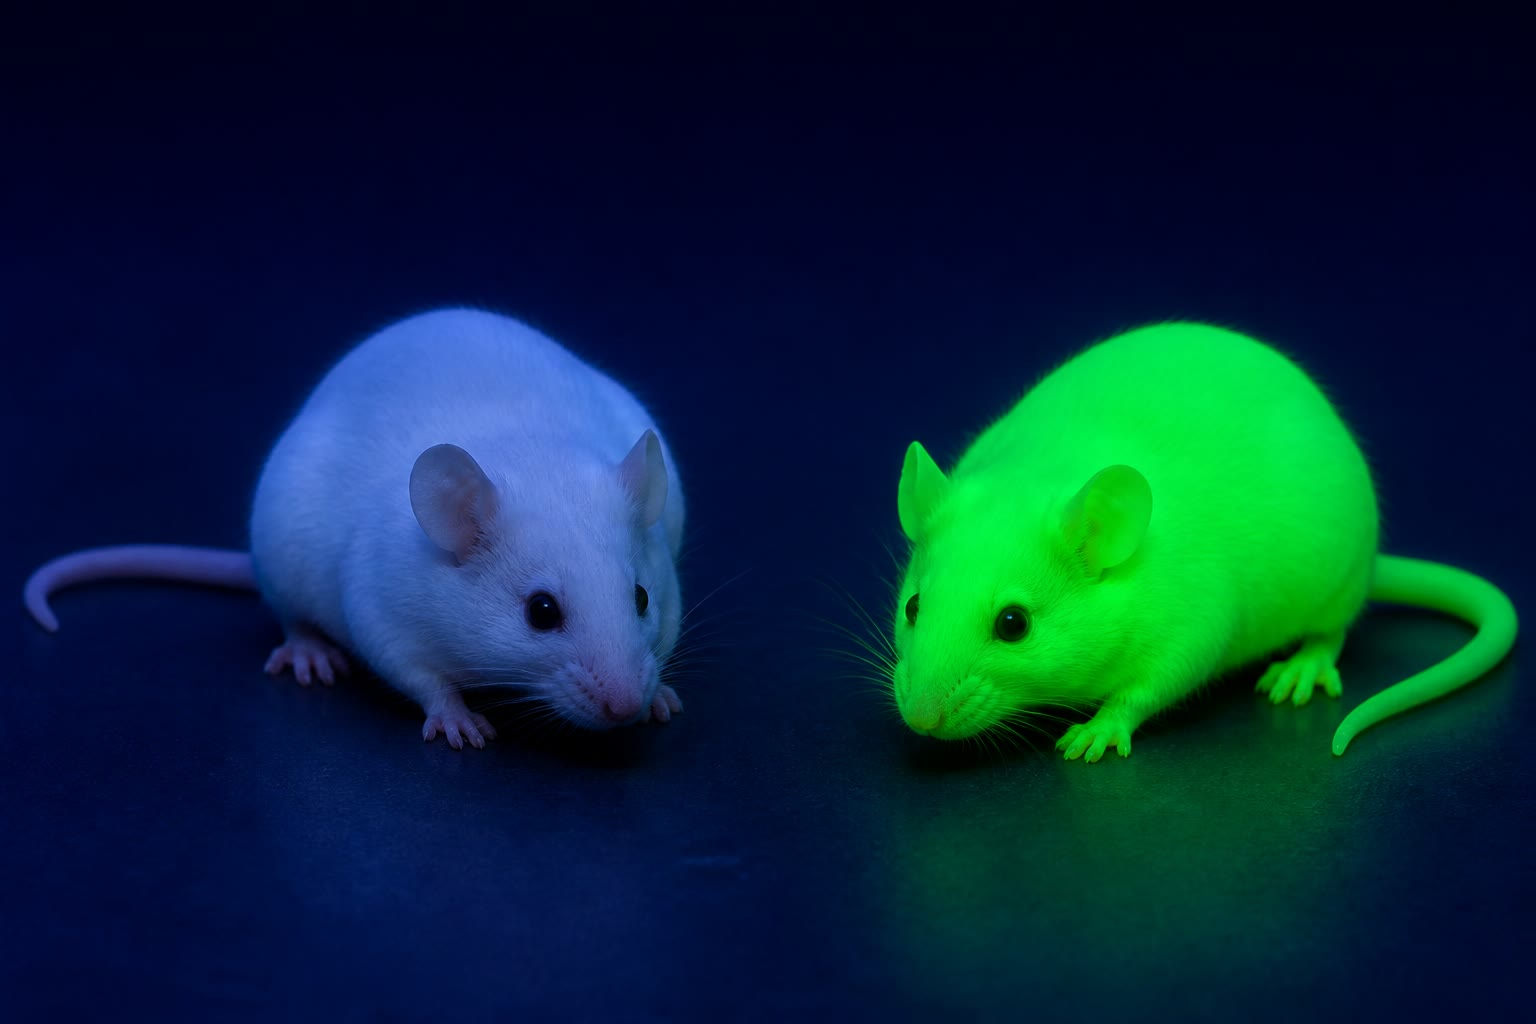
\includegraphics[width=0.62\linewidth]{images/book2/ai/g10-dna-gfp-mice.jpg}

{\small नीले प्रकाश में, जेलीफ़िश का हरे प्रतिदीप्त \omterm{def:g10:chemistry-of-life:families}{प्रोटीन} वाला \omterm{def:g10:universal-dna:gene}{जीन} ढोता
एक चूहा किसी साधारण चूहे के पास हरा चमक रहा है। वही अणु, वही पढ़ने के
नियम: जेलीफ़िश का निर्देश चूहे में चल रहा है।}
\end{omfigure}

\begin{example}[पारजीनन के उपयोग]\label{ex:g10:universal-dna:uses}
जीवाणुओं से बना मानव इंसुलिन और वृद्धि हॉर्मोन; मक्का या कपास में डाला
गया किसी कीट-पीड़क के प्रति प्रतिरोध का \omterm{def:g10:universal-dna:gene}{जीन}; विटामिन A के पूर्ववर्ती को
बनाने वाले \omterm{def:g10:universal-dna:gene}{जीन} ढोता चावल; और किसी दूसरे \omterm{def:g10:universal-dna:gene}{जीन} के साथ जोड़ा गया GFP \omterm{def:g10:universal-dna:gene}{जीन},
ताकि जिन \omterm{def:g10:cells-common-unit:cell}{कोशिकाओं} में वह \omterm{def:g10:universal-dna:gene}{जीन} सक्रिय हो वे सूक्ष्मदर्शी के नीचे जल उठें
--- यह आख़िरी उपयोग, यानी शोध का एक औज़ार, सबसे आम है। हर उपयोग सुरक्षा
के और पर्यावरण पर पड़ने वाले असर के अपने सवाल खड़े करता है; और हर उपयोग
उसी एक तथ्य पर टिका है, यानी आनुवंशिक अणु की सार्वत्रिकता पर।
\end{example}

\begin{remark}[अणुओं के स्तर पर एकता और विविधता]\label{rem:g10:universal-dna:unity}
\omterm{def:g10:universal-dna:information}{DNA} की सार्वत्रिकता \cref{ch:g10:chemistry-of-life} में मिली जीवन की उसी
एकता का आणविक चेहरा है: पृथ्वी के हर जीव के लिए एक रसायन, एक ही
जानकारी-अणु, एक ही पढ़ने की व्यवस्था --- और साझा उद्गम की भविष्यवाणी ठीक
यही है (\cref{ch:g10:common-ancestry})। जीवन की विविधता भी उसी अणु में
लिखी है, अनुक्रम के फ़र्क़ों के रूप में: दो विकल्पियों के बीच चंद \omterm{def:g10:universal-dna:nucleotide}{क्षारक},
दो जातियों के बीच जीनोम का कुछ प्रतिशत, और किसी जीवाणु तथा मनुष्य के बीच
उस पूरी इबारत का संगठन।
\end{remark}

\section{अभ्यास}

\begin{exercise}[$\star$]\label{exo:g10:universal-dna:1}
\omterm{def:g10:universal-dna:nucleotide}{न्यूक्लियोटाइड} के तीन हिस्सों और \omterm{def:g10:universal-dna:information}{DNA} के चारों \omterm{def:g10:universal-dna:nucleotide}{क्षारकों} के नाम लिखिए।
\end{exercise}

\begin{exercise}[$\star$]\label{exo:g10:universal-dna:2}
\texttt{TACGGATTCA} की पूरक लड़ी लिखिए।
\end{exercise}

\begin{exercise}[$\star$]\label{exo:g10:universal-dna:3}
किसी \omterm{def:g10:universal-dna:information}{DNA} नमूने में 21\% ग्वानीन है। C, A और T के प्रतिशत बताइए।
\end{exercise}

\begin{exercise}[$\star$]\label{exo:g10:universal-dna:4}
\omterm{def:g10:universal-dna:gene}{जीन} और \omterm{def:g10:universal-dna:gene}{युग्मविकल्पी} की एक-एक वाक्य में परिभाषा दीजिए, और उसमें
``अनुक्रम'' शब्द का इस्तेमाल कीजिए।
\end{exercise}

\begin{exercise}[$\star$]\label{exo:g10:universal-dna:5}
पारजीनी जीव क्या होता है? अध्याय से उसके दो उदाहरण दीजिए।
\end{exercise}

\begin{exercise}[$\star\star$]\label{exo:g10:universal-dna:6}
कोई \omterm{def:g10:universal-dna:gene}{जीन} 1500 क्षारक-जोड़े लंबा है। नैनोमीटर में उसकी लंबाई क्या है, और
वह कुंडली के कितने चक्कर बनाता है?
\end{exercise}

\begin{exercise}[$\star\star$]\label{exo:g10:universal-dna:7}
मानव की एक \omterm{def:g10:cells-common-unit:cell}{कोशिका} में \omterm{def:g10:universal-dna:information}{DNA} की कुल लंबाई निकालिए, यह देते हुए कि
\omterm{def:g10:universal-dna:information}{गुणसूत्रों} के प्रति समुच्चय $\num{3.2e9}$ क्षारक-जोड़े हैं और प्रति
\omterm{def:g10:cells-common-unit:cell}{कोशिका} दो समुच्चय। \omterm{def:g10:cells-common-unit:organelle}{केंद्रक} के व्यास \qty{6}{\micro m} से तुलना कीजिए।
\end{exercise}

\begin{exercise}[$\star\star$]\label{exo:g10:universal-dna:8}
एवरी के प्रयोग में \omterm{def:g10:universal-dna:information}{DNA} को नष्ट करने वाले एंजाइम से उपचारित सत्त को भी
परखना क्यों ज़रूरी था, केवल शुद्ध किया गया \omterm{def:g10:universal-dna:information}{DNA} वाला अंश ही क्यों नहीं?
\end{exercise}

\begin{exercise}[$\star\star$]\label{exo:g10:universal-dna:9}
समझाइए कि शारगाफ़ के आँकड़ों ने ऐसे मॉडल को क्यों ख़ारिज कर दिया जिसमें
\omterm{def:g10:universal-dna:nucleotide}{क्षारक} \texttt{ATGCATGC\dots} जैसे नियमित दोहराव में सजे होते।
\end{exercise}

\begin{exercise}[$\star\star$]\label{exo:g10:universal-dna:10}
किसी \omterm{def:g10:universal-dna:gene}{जीन} के दो \omterm{def:g10:universal-dna:gene}{युग्मविकल्पी} 2000 में से एक ही \omterm{def:g10:universal-dna:nucleotide}{क्षारक} पर अलग हैं। समझाइए कि
इतना छोटा फ़र्क़ किसी \omterm{def:g10:chemistry-of-life:families}{प्रोटीन} को कैसे बदल सकता है, और वह कुछ भी क्यों न
बदले, यह भी।
\end{exercise}

\begin{exercise}[$\star\star$]\label{exo:g10:universal-dna:11}
चूहे के निषेचित अंडाणु में डाला गया GFP \omterm{def:g10:universal-dna:gene}{जीन} उसकी त्वचा की \omterm{def:g10:cells-common-unit:cell}{कोशिकाओं} में,
यकृत की \omterm{def:g10:cells-common-unit:cell}{कोशिकाओं} में और शुक्राणुओं में मिलता है। \omterm{def:g10:cells-common-unit:cell}{कोशिका} सिद्धांत और
\cref{prop:g10:universal-dna:explains} की मदद से समझाइए कि ऐसा क्यों है।
\end{exercise}

\begin{exercise}[$\star\star\star$]\label{exo:g10:universal-dna:12}
किसी जीवाणु का \omterm{def:g10:universal-dna:information}{DNA} अणु $\num{4.6e6}$ क्षारक-जोड़े लंबा है। उसकी लंबाई
निकालिए; \omterm{def:g10:cells-common-unit:cell}{कोशिका} के \qty{2}{\micro m} से तुलना कीजिए; फिर समझाइए कि इसके
बावजूद जीवाणु में उसके लिए जगह कैसे बन जाती है।
\end{exercise}

\begin{exercise}[$\star\star\star$]\label{exo:g10:universal-dna:13}
कोई मित्र दावा करता है कि मानव \omterm{def:g10:universal-dna:information}{DNA} जीवाणु के \omterm{def:g10:universal-dna:information}{DNA} से ``अधिक जटिल'' ज़रूर
होगा, क्योंकि उसमें अधिक \omterm{def:g10:universal-dna:nucleotide}{क्षारक} हैं। $\num{3.2e9}$ और $\num{4.6e6}$
क्षारक-जोड़ों की तुलना $\num{20000}$ और 4300 \omterm{def:g10:universal-dna:gene}{जीनों} से कीजिए, और चर्चा
कीजिए कि वह अतिरिक्त \omterm{def:g10:universal-dna:information}{DNA} क्या है और क्या नहीं।
\end{exercise}

\begin{exercise}[$\star\star\star$]\label{exo:g10:universal-dna:14}
मान लीजिए कोई ऐसी जाति खोजी जाती है जिसका आनुवंशिक पदार्थ किसी और अणु और
किसी और कूट का इस्तेमाल करता हो। वह अध्याय की किन प्रतिज्ञप्तियों का
खंडन करती, और उस जाति तथा बाक़ी जीवन के साझा उद्गम के लिए उसका क्या
मतलब होता?
\end{exercise}

\begin{exercise}[$\star\star\star$]\label{exo:g10:universal-dna:15}
जीवाणुओं से बने मानव इंसुलिन ने सूअरों के अग्न्याशय से निकाले जाने वाले
इंसुलिन की जगह ले ली। जीवाणु वाला उत्पाद बेहतर क्यों था, इसके दो जैविक
कारण गिनाइए, और एक ऐसा सवाल भी जो किसी नियामक को फिर भी पूछना पड़ता।
\end{exercise}

\section{समस्या: जेलीफ़िश का जीन}

\begin{problem}[{सप्ताहांत समस्या --- जेलीफ़िश का एक जीन चूहे तक पीछा
किया गया: उसकी लंबाई, उसके अक्षर, चूहा उसे पढ़ क्यों सकता है, और वे दो
मीटर DNA जो उसे हर कोशिका में ढोते हैं}]
\label{pb:g10:universal-dna:1}
जेलीफ़िश \emph{Aequorea victoria} का हरा प्रतिदीप्त \omterm{def:g10:chemistry-of-life:families}{प्रोटीन} 238 \omterm{def:g10:chemistry-of-life:families}{ऐमीनो
अम्लों} की एक शृंखला है। प्रयोगशाला में इस्तेमाल होने वाला उसका \omterm{def:g10:universal-dna:gene}{जीन} 720
क्षारक-जोड़ों का एक \omterm{def:g10:universal-dna:information}{DNA} खंड है। प्रति क्षारक-जोड़ा \qty{0.34}{nm}, प्रति
चक्कर दस क्षारक-जोड़े, और चूहे का जीनोम \omterm{def:g10:universal-dna:information}{गुणसूत्रों} के प्रति समुच्चय
$\num{2.7e9}$ क्षारक-जोड़े तथा प्रति \omterm{def:g10:cells-common-unit:cell}{कोशिका} दो समुच्चय लीजिए।

\medskip
\noindent\textbf{भाग I --- अणु।}
\begin{enumerate}
  \item GFP \omterm{def:g10:universal-dna:gene}{जीन} की लंबाई नैनोमीटर में और उसके बनाए कुंडली के चक्करों की
        संख्या निकालिए।
  \item \omterm{def:g10:universal-dna:gene}{जीन} की एक लड़ी \texttt{ATGAGTAAAGGAGAAGAAC} से शुरू होती है।
        उसकी पूरक लड़ी लिखिए।
  \item पूरे \omterm{def:g10:universal-dna:gene}{जीन} में एडेनीन \omterm{def:g10:universal-dna:nucleotide}{क्षारकों} का 27\% है। बाक़ी तीनों \omterm{def:g10:universal-dna:nucleotide}{क्षारकों} के
        प्रतिशत बताइए।
  \item \omterm{def:g10:universal-dna:gene}{जीन} में 720 क्षारक-जोड़े हैं और वह 238 \omterm{def:g10:chemistry-of-life:families}{ऐमीनो अम्लों} का कूट है।
        अनुपात निकालिए, और सुझाइए कि इससे एक \omterm{def:g10:chemistry-of-life:families}{ऐमीनो अम्ल} कितने \omterm{def:g10:universal-dna:nucleotide}{क्षारकों}
        से तय होता है इस बारे में क्या पता चलता है (यह परिकल्पना
        \cref{ch:g11:gene-expression} पक्की करेगा)।
  \item सिद्धांततः 720 \omterm{def:g10:universal-dna:nucleotide}{क्षारकों} के कितने अलग-अलग अनुक्रम संभव हैं? उत्तर
        4 की घात के रूप में लिखिए, फिर एक वाक्य में समझाइए कि उस अनुक्रम
        को जानकारी क्यों कहा जा सकता है।
\end{enumerate}

\medskip
\noindent\textbf{भाग II --- चूहा उसे पढ़ क्यों सकता है।}
\begin{enumerate}[resume]
  \item \omterm{def:g10:universal-dna:information}{DNA} का वह गुण बताइए जिसकी वजह से चूहे की \omterm{def:g10:cells-common-unit:cell}{कोशिका} जेलीफ़िश के \omterm{def:g10:universal-dna:gene}{जीन}
        का इस्तेमाल कर पाती है।
  \item \omterm{def:g10:universal-dna:gene}{जीन} किसी वयस्क चूहे की त्वचा में नहीं, बल्कि निषेचित अंडाणु में
        डाला जाता है। \omterm{def:g10:cells-common-unit:cell}{कोशिका} सिद्धांत की मदद से समझाइए कि इससे \omterm{def:g10:universal-dna:gene}{जीन} कहाँ
        पहुँचेगा, इस पर क्या फ़र्क़ पड़ता है।
  \item वयस्क चूहा हर ऊतक में चमकता है। इससे उसकी अलग-अलग तरह की
        \omterm{def:g10:cells-common-unit:cell}{कोशिकाओं} की DNA-मात्रा के बारे में क्या पता चलता है?
  \item चमकते चूहे का संगम किसी साधारण चूहे से कराया जाता है। कारण सहित
        अनुमान लगाइए कि संतानों में से कुछ चमकेंगी या नहीं।
  \item एक नियंत्रण चूहे में \omterm{def:g10:universal-dna:gene}{जीन} के बजाय शुद्ध किया गया GFP \omterm{def:g10:chemistry-of-life:families}{प्रोटीन}
        इंजेक्ट किया जाता है: वह कुछ दिन फीका चमकता है, फिर रुक जाता है।
        दोनों प्रयोगों का अंतर समझाइए।
\end{enumerate}

\medskip
\noindent\textbf{भाग III --- कहानी के पीछे का साक्ष्य।}
\begin{enumerate}[resume]
  \item एवरी के प्रयोग में उस अंश का नाम बताइए जिसने जीवाणुओं को
        रूपांतरित किया, और उस उपचार का भी जिसने रूपांतरण मिटा दिया।
  \item समझाइए कि रूपांतरण का प्रयोग \omterm{prop:g10:universal-dna:universal}{पारजीनन} का ही एक प्राकृतिक रूप
        क्यों है।
  \item शारगाफ़ ने हर जाति में A$\,=\,$T और G$\,=\,$C पाया, पर A+T 25\%
        से 75\% तक बदलता हुआ। दोनों प्रेक्षणों में से कौन-सा
        क्षारक-जोड़ी का समर्थन करता है, और कौन-सा दिखाता है कि अनुक्रम
        स्वतंत्र है?
  \item फ़्रैंकलिन के चित्रों ने कुंडली का व्यास \qty{2}{nm} बताया।
        समझाइए कि किसी बड़े \omterm{def:g10:universal-dna:nucleotide}{क्षारक} को किसी छोटे के साथ जोड़ने (A को T के
        साथ, G को C के साथ) से, न कि दो बड़ों को आपस में, कुंडली नियमित
        क्यों बनती है।
  \item बनावट की खोज ने तुरंत यह क्यों सुझा दिया कि \omterm{def:g10:universal-dna:information}{DNA} की नक़ल कैसे
        बनती है?
\end{enumerate}

\medskip
\noindent\textbf{भाग IV --- किसी \omterm{def:g10:cells-common-unit:organelle}{केंद्रक} में दो मीटर।}
\begin{enumerate}[resume]
  \item चूहे की एक \omterm{def:g10:cells-common-unit:cell}{कोशिका} में \omterm{def:g10:universal-dna:information}{DNA} की कुल लंबाई निकालिए।
  \item \omterm{def:g10:cells-common-unit:organelle}{केंद्रक} \qty{6}{\micro m} चौड़ा है। समा जाने के लिए \omterm{def:g10:universal-dna:information}{DNA} को
        कुंडलन से कितने गुना छोटा होना पड़ेगा?
  \item \omterm{def:g10:cells-common-unit:cell}{कोशिका} के \omterm{def:g10:universal-dna:information}{DNA} का कितना अंश GFP \omterm{def:g10:universal-dna:gene}{जीन} है?
  \item चूहे में लगभग $\num{2e4}$ \omterm{def:g10:universal-dna:gene}{जीन} हैं, जिनकी औसत लंबाई अकूट हिस्सों
        समेत $\num{3e4}$ क्षारक-जोड़े है। \omterm{def:g10:universal-dna:gene}{जीन} जीनोम का कितना अंश घेरते
        हैं?
  \item परिणाम एक वाक्य में लिखिए: चूहे की एक \omterm{def:g10:cells-common-unit:cell}{कोशिका} कितना \omterm{def:g10:universal-dna:information}{DNA} ढोती है,
        और उस \omterm{def:g10:universal-dna:information}{DNA} के बारे में वह अकेला कौन-सा तथ्य है जिसकी वजह से उसके
        हज़ारों \omterm{def:g10:universal-dna:gene}{जीनों} के बीच जेलीफ़िश का एक \omterm{def:g10:universal-dna:gene}{जीन} पढ़ा जा सकता है?
\end{enumerate}
\end{problem}
